\chapter{Imagerie radiale}
\setlength{\footskip}{50pt}
\label{Chap2}
\section{Description de l'espace de Fourier}

Une expérience de RMN élémentaire standard nous permet de mesurer un signal provenant d'un volume mais il est impossible d'assigner une position spatiale aux protons à partir de ce seul signal. Cependant, l'information spatiale peut être indirectement obtenue en répétant cette expérience élémentaire avec l'application supplémentaire de différentes combinaisons de gradients de champs magnétiques dans 2 ou 3 directions. Les signaux recueillis peuvent alors être stockés dans une matrice que l'on appelle espace de Fourier (ou espace-K) à partir de laquelle une opération mathématique (Transformée de Fourier) permettra d'obtenir une image. 
Généralement, la construction d'une image nécessite le recueil d'une série de signaux appelés acquisitions. Pour chaque acquisition, une impulsion radiofréquence (RF) engendre une nouvelle valeur d'aimantation transverse à l'origine du signal et qui est alors échantillonnée selon une trajectoire particulière de l'espace de Fourier (figure \ref{fig:Signal2Image}).


\begin{figure}[h]
\centering
\line(1,0){400} \\
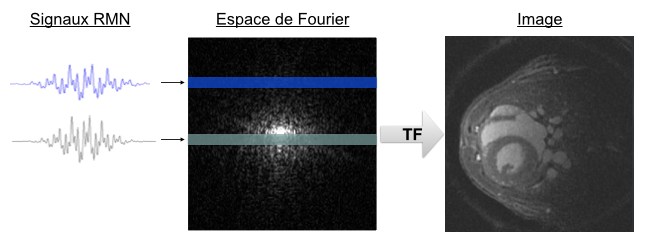
\includegraphics[scale=0.7]{./figure/chap2/Signal2Image.png}
\caption[Formation d'une image à partir de signal RMN.]{\label{fig:Signal2Image} \textbf{Formation d'une image à partir du signal RMN.} Les signaux recueillis sont stockés dans l'espace de Fourier qui après une transformée de Fourier (TF) permet d'obtenir une image.}
\line(1,0){400} \\
\end{figure}

%V11 mars 2015. En principe, une image complète d'IRM peut être reconstruite à partir d'une seule acquisition en utilisant une trajectoire qui  parcoure tout l'espace de Fourier. C'est une méthode très souvent utilisé en imagerie fonctionnelle. Cependant, pour la plupart des applications cela entraine l'apparition d'artefacts dans l'image et d'une faible résolution spatial. Cela est due à la décroissance exponentielle du signal qui limite la fenêtre de temps d'acquisition exploitable. Mais cette fenêtre d'acquisition est aussi dicté par la performance du système de gradient et les contraintes physiologiques qui limite la vitesse à laquelle l'espace de Fourier peut être traversé. Il en résulte que la plupart des méthodes d'imagerie IRM utilisent de multiple acquisitions, chacune d'entre elles permettant de recueillir les informations d'une partie de l'espace de Fourier.

En principe, une image complète d'IRM peut être reconstruite à partir d'une seule acquisition en utilisant une trajectoire qui  parcourt tout l'espace de Fourier. Cependant, pour la plupart des applications cela entraîne l'apparition d'artefacts dans l'image et d'une faible résolution spatiale. Cela est dû à la décroissance exponentielle du signal qui limite la fenêtre de temps d'acquisition exploitable. Mais cette fenêtre d'acquisition est aussi dictée par la performance du système de gradient et les contraintes physiologiques qui limitent la vitesse à laquelle l'espace de Fourier peut être parcouru. Il en résulte que la plupart des méthodes d'imagerie IRM utilisent de multiples acquisitions, chacune d'entre elles permettant de recueillir les informations d'une partie de l'espace de Fourier.

Une partie du développement de nouvelles méthodes d'acquisition en IRM consiste à modifier la stratégie et les trajectoires permettant de remplir l'espace de Fourier.


\subsection{Parcours de l'espace de Fourier}
\label{subsec:Parcours}

Un déplacement dans l'espace de Fourier s'effectue grâce à l'application des gradients de codage de l'espace. L'application d'un gradient induit en effet une variation de la fréquence de précession des spins dépendante de leurs positions dans l'espace. Suite à l'arrêt des gradients, les spins précessent à nouveau à la même fréquence mais ont accumulé une différence de phase qui dépend de leur position par rapport à l'isocentre de l'imageur. Le signal mesuré provenant de l'ensemble des ces spins est stocké dans l'espace de Fourier aux coordonnées définies par l'équation :
\begin{equation}
\overrightarrow{k(T)}= \frac{\gamma}{2\pi} \int_0^T \overrightarrow{G(t)}dt
\end{equation}

Le déplacement entre deux points de l'espace de Fourier est proportionnel à l'aire de l'ensemble des gradients appliqués, plus l'aire est importante plus la distance parcourue entre deux points le sera aussi. En appliquant des gradients selon des axes différents, il est possible de parcourir l'espace de Fourier en 2D comme dans la figure \ref{fig:ParcoursKspace} ou en 3D avec l'ajout d'un axe de gradient supplémentaire.

\begin{figure}[H]
\centering
\line(1,0){400} \\
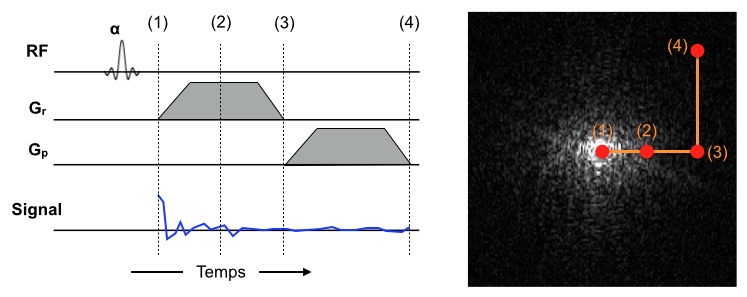
\includegraphics[scale=0.6]{./figure/chap2/ParcoursKspace.png}
\caption[Parcours de l'espace de Fourier en fonction de l'application de gradients.]{\label{fig:ParcoursKspace} \textbf{Parcours de l'espace de Fourier en fonction de l'application de gradients.} Après l'impulsion radiofréquence d'angle $\alpha$, l'espace de Fourier est parcouru suivant un axe horizontal grâce au gradient appliqué sur l'axe $G_r$ puis selon un axe vertical grâce à l'application d'un gradient sur l'axe $G_p$. Les positions des points 1 à 4 dans l'espace de Fourier sont indiqués sur le chronogramme.}
\line(1,0){400} \\
\end{figure}


\subsection{Propriétés de l'espace de Fourier}

L'espace de Fourier, de par sa nature, dispose de nombreuses propriétés qui peuvent être exploitées lors du développement de nouvelles méthodes d'acquisition. 

\subsubsection{Régions centrale et extérieure}
\label{subsec:KSpaceRegion}
Les régions centrale et périphérique de l'espace de Fourier contribuent différemment à la construction de l'image. La figure \ref{fig:kSpaceResSig} illustre le fait que le centre de l'espace contient les basses fréquences de l'image et renseigne principalement sur le signal et le contraste, alors que la périphérie encodant les hautes fréquences spatiales renseigne quant à elles sur les détails, les contours ainsi que le bruit.

\begin{figure}[H]
\centering
\line(1,0){400} \\
\includegraphics[scale=0.7]{./figure/chap2/kSpaceResSig.png}
\caption[Contribution des données de l'espace de Fourier en fonction de leur position.]{\label{fig:kSpaceResSig} \textbf{Contribution des données de l'espace de Fourier en fonction de leur position.} Les régions centrale et/ou périphérique de l'espace de Fourier sont utilisées pour reconstruire les images grâce à une transformée de Fourier. La reconstruction avec le centre de l'espace donne une image floue mais contrastée alors que la périphérie de l'espace donne une image détaillée mais avec peu de signal et de contraste.}
\line(1,0){400} \\
\end{figure}

\subsubsection{Résolution et champ de vue}

La résolution de l'image est donnée par la taille de l'espace de Fourier qui est échantillonné; plus celle-ci est grande plus l'image sera résolue.
\begin{equation}
\Delta x = \frac{1}{2*k_{max}}
\end{equation}
où $k_{max}$ est la position du point échantillonné la plus éloignée du centre de l'espace de Fourier. Le champ de vue est quant à lui déterminé par la densité d'échantillonnage de cette région. Pour obtenir un grand champ de vue, notée ici FOV (Field of view), il faut échantillonner de manière dense l'espace de Fourier. Le FOV est relié à la distance d'échantillonage $\delta k$ par la relation suivante :
\begin{equation}
\label{eq:FOV}
FOV = \frac{1}{\Delta k}
\end{equation}
Généralement, l'espace de Fourier est échantillonné de manière à respecter le critère de Nyquist selon lequel la fréquence d'échantillonnage (1/$\delta t$) doit être au moins 2 fois supérieure à la plus haute fréquence contenue dans le signal. Ce critère aboutit à la relation :
\begin{equation}
\Delta k =\frac{2k_{max}}{n} \leq \frac{1}{FOV}
\end{equation}
où $n$ correspond au nombre de points échantillonnés pour une acquisition. Une violation du critère de Nyquist créera des artefacts dans l'image dépendant du type de trajectoire utilisé pour échantillonner l'espace de Fourier (figure \ref{fig:Undersamp}).
\begin{figure}[H]
\centering
\line(1,0){400} \\
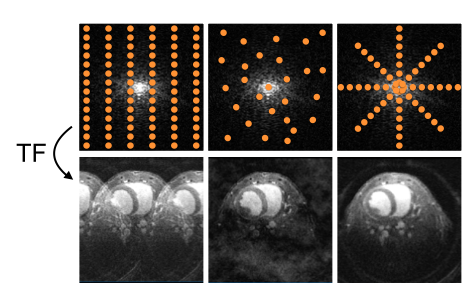
\includegraphics[scale=1]{./figure/chap2/Undersamp.png}
\caption[Sous-échantillonnage de l'espace de Fourier.]{\label{fig:Undersamp} \textbf{Sous-échantillonnage de l'espace de Fourier.} La violation du critère de Nyquist introduit des artefacts dans le domaine image qui dépendent de la trajectoire utilisée. A gauche : Avec une fréquence d'échantillonnage insuffisante d'un facteur 2 pour une acquisition cartésienne, on observe des artefacts de repliement. Au milieu : avec un espace sous-échantillonné aléatoirement avec un facteur 2, on observe des artefacts incohérents. A droite : avec un espace sous-échantillonné 5 fois avec des trajectoires radiales, on observe une diminution de la résolution.}
\line(1,0){400} \\
\end{figure}

\subsection{Trajectoire d'échantillonnage}

La trajectoire la plus couramment utilisée est la trajectoire cartésienne qui consiste en l'acquisition de lignes parallèles de l'espace de Fourier (figure \ref{fig:TrajCart}). Cela s'explique par sa reconstruction extrêmement simple, rapide et robuste qui utilise la Transformée de Fourier Rapide (notée FFT pour "Fast Fourier Transform"), un algorithme de calcul de la transformée de Fourier discrète. Et surtout, la reconstruction à partir de cette trajectoire est peu sensible à de nombreuses sources d'imperfections. Le principal problème de ce schéma d'acquisitions est sa sensibilité au mouvement et ses artefacts cohérents de repliement qui sont créés en cas de sous-échantillonnage.
%%%%%Modif 08/03/2015
%Cependant, la conception d'une trajectoire est relativement libre et peut permettre d'obtenir certaines propriétés intéressante que ce soit en terme de temps, d'acquisition, faible sensibilité aux mouvement ou pour des applications spécifiques. 
Bien que ces schémas de trajectoires soient majoritairement employés, de nombreux autres ont été développés et sont décrits dans la littérature. Parmis ceux-ci, les trajectoires radiales ont des propriétés intéressantes pour des applications sur le petit animal.

\begin{figure}[h]
\centering
\line(1,0){400} \\
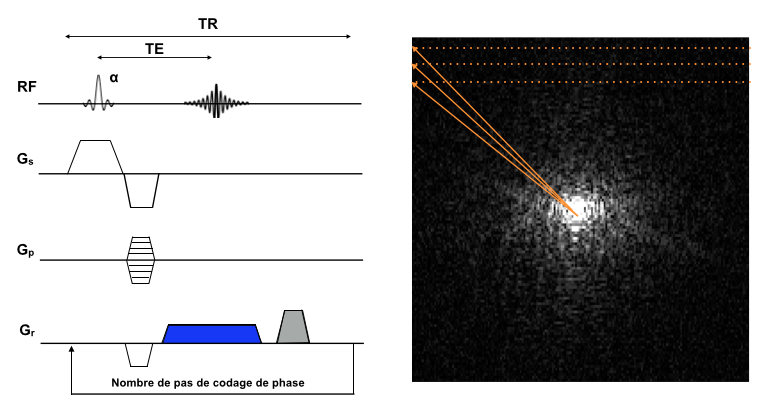
\includegraphics[scale=0.5]{./figure/chap2/TrajCart.png}
\caption[Chronogramme d'une séquence cartésienne.]{\label{fig:TrajCart} \textbf{Chronogramme d'une séquence cartésienne.} Pour les trajectoires cartésiennes, la lecture du signal s'effectue durant l'application d'un gradient de lecture constant (selon $G_r$). Les autres gradients servent à positionner le premier point de la lecture après l'impulsion radiofréquence qui bascule l'aimantation dans le plan transverse.}
\line(1,0){400} \\
\end{figure}

\section{Trajectoire radiale dans l'espace de Fourier}

\subsection{Principe}
Le schéma d'acquisition radiale a tout d'abord été proposé par Lauterbur en 1973 \cite{lauterbur1973image}. Peu après l'introduction des scanners commerciaux, les trajectoires radiales ont été remplacées par des trajectoires cartésiennes car celles-ci étaient plus robustes aux hétérogénéités de champs $B_0$ et à la non-linéarité des gradients qui étaient très présents sur les premiers scanners IRM. Au fil des années, un regain d'intérêt est apparu pour les séquences radiales grâce aux progrès techniques en particulier sur la compensation des courants de Foucault dans les gradients et la meilleure homogénéité du champ statique. 

En imagerie radiale, le signal IRM est échantillonné selon des trajectoires suivant les rayons ou les diamètres d'un disque qui permettent d'obtenir respectivement une séquence à temps d'écho ultra-court (UTE) ou une séquence projection-reconstruction (PR). Dans le cas d'une séquence 2D la trajectoire est inscrite dans un disque et, pour les séquence 3D, dans une sphère. Les différentes trajectoires sont illustrées sur la figure \ref{fig:TrajRad}.

\begin{figure}[H]
\centering
\line(1,0){400} \\
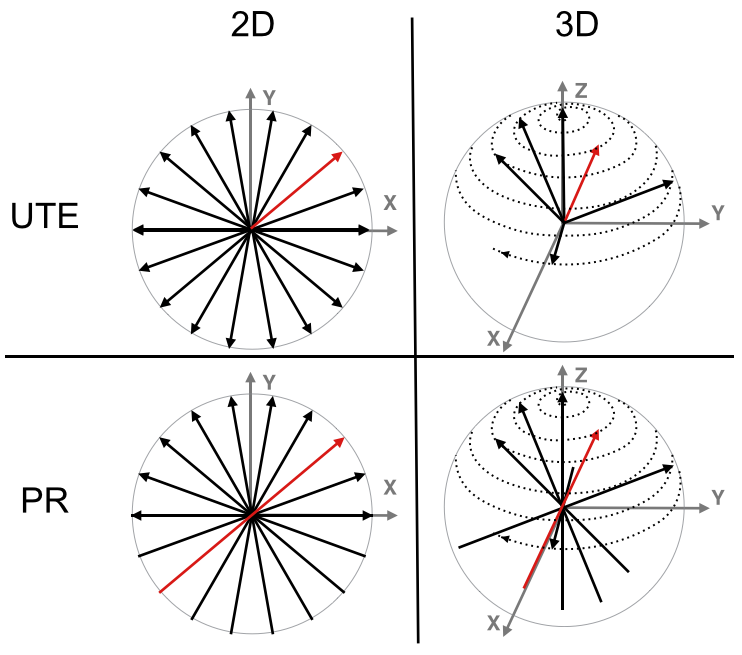
\includegraphics[scale=0.5]{./figure/chap2/TrajRad.png}
\caption[Représentation des types de trajectoires radiales.]{\label{fig:TrajRad} \textbf{Représentation des types de trajectoires radiales.} Les trajectoires radiales 2D et 3D sont représentées schématiquement dans le cas d'une acquisition UTE ou PR.}
\line(1,0){400} \\
\end{figure}




\subsection{Description mathématique}

Pour recueillir le signal selon les trajectoires radiales, l'amplitude des gradients varie selon les 3 axes simultanément selon l'équation :
\begin{equation}
\label{eq:AngleRadial}
\begin{split}
	G_x & =G\cos(\phi)\sin(\theta)\\
	G_y & =G\sin(\phi)\sin(\theta)\\	
	G_z & =G\cos(\theta)
\end{split}
\end{equation}
où $\theta$ et $\phi$ correspondent aux angles définis dans la figure \ref{fig:SphereCoord}.
Puisque les gradients dans les 3 directions sont utilisés pour chaque acquisition radiale de l'espace de Fourier, ils sont considérés comme des gradients de lecture plutôt que des gradients d'encodage de fréquence et de phase comme pour une acquisition cartésienne. Dans le cas d'une acquisition 2D, seul l'angle $\theta = \frac{\pi}{2}$ est utilisé ce qui a pour conséquence de fixer la valeur du gradient z à 0 et de ne faire varier les gradients que selon les axes x et y en fonction des valeurs de $\phi$.

\begin{figure} [H]
\centering
\line(1,0){400} \\
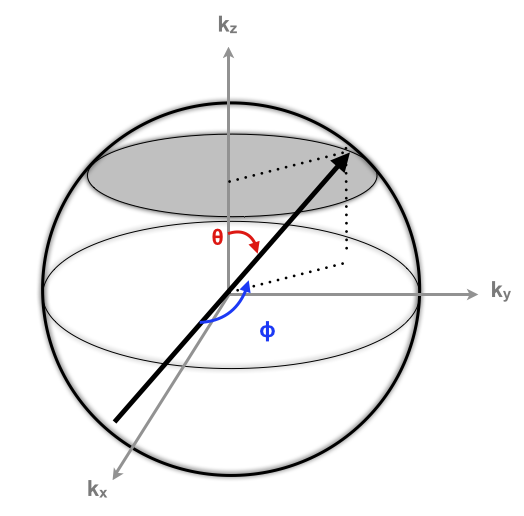
\includegraphics[scale=0.5]{./figure/chap2/SphereCoord.png}
\caption[Définition des coordonnées sphériques.]{\label{fig:SphereCoord} \textbf{Définition des coordonnées sphériques.} Représentation des angles $\theta$ et $\Phi$ utilisés  pour définir les trajectoires radiales en 3 dimensions.}
\line(1,0){400} \\
\end{figure}

Comme pour le cas cartésien, la distance entre deux points échantillonnés sur une projection est généralement définie par la taille du FOV désiré grâce à l'équation \ref{eq:FOV} et n, le nombre de points échantillonnés est défini par la résolution de base désirée. Avec une trajectoire radiale, ces deux paramètres ne sont pas suffisants pour définir la résolution spatiale réelle de l'image car celle-ci dépend aussi de $n_p$, le nombre de projections utilisé. Pour satisfaire le critère de Nyquist, d'après la littérature \cite{bernstein2004handbook}, il est nécessaire d'utiliser un nombre de projections égal à :
\begin{equation}
\label{eq:NyquistRad}
\begin{aligned}
	(2D)\;\;\;\; n_p = \frac{\pi}{2} \times n \\
	(3D)\;\ \ n_p = \pi \times n^2 
\end{aligned}
\end{equation}
qui assure que la distance entre deux points de projections voisines soit inférieure ou égale à $\Delta k$.

\subsection{Chronogramme des séquences}

Comme décrit dans la partie \ref{subsec:Parcours}, une trajectoire dans l'espace de Fourier correspond à l'application de gradient avec une intensité donnée selon un ordre chronologique. Pour représenter une séquence, il est courant d'utiliser un chronogramme qui présente entre autre les gradients de lecture, de phase et de sélection de coupe que l'on notera respectivement $G_r$, $G_p$ et $G_s$ ainsi que les impulsions RF. Les chronogrammes de la séquence radiale 3D PR et UTE sont présentés dans la figure \ref{fig:KspacePR}.

\begin{figure}[h]
\centering
\line(1,0){400} \\
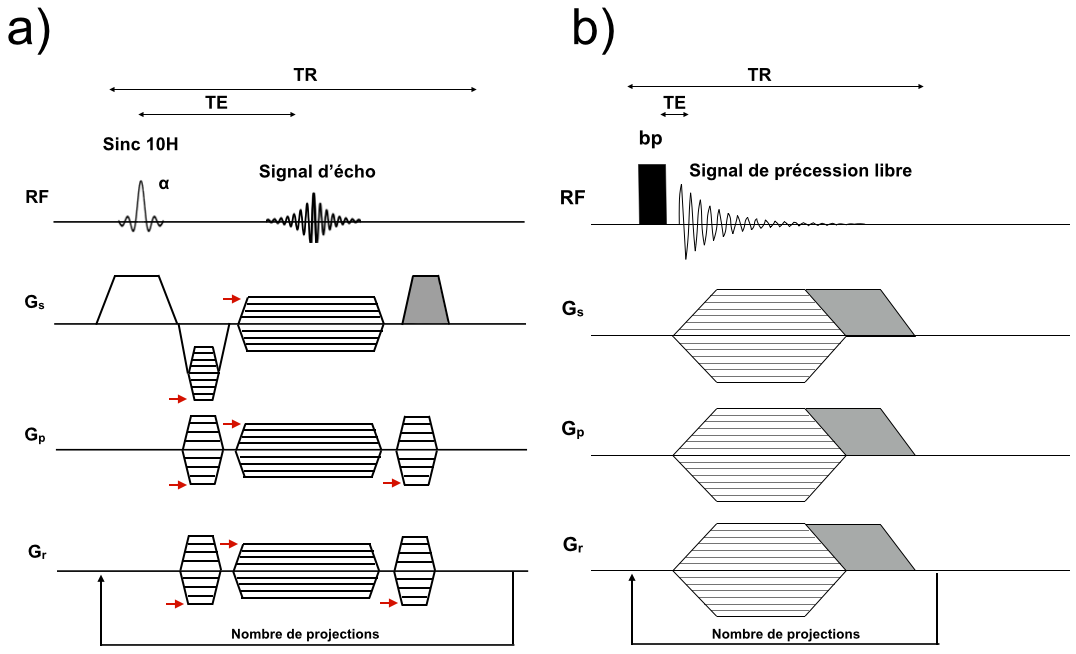
\includegraphics[scale=0.4]{./figure/chap2/KspacePR.png}
\caption[Chronogramme des séquences radiales.]{\label{fig:KspacePR} \textbf{Chronogramme des séquences radiales.} (a) Chronogramme d'une séquence radiale 3D PR. (b) Chronogramme d'une séquence radiale 3D UTE. Les gradients grisés permettent de déphaser l'aimantation transverse résiduelle avant la prochaine excitation radiofréquence.} 
\line(1,0){400} \\
\end{figure}

La séquence PR débute avec une impulsion RF qui peut être sélective grâce à l'application d'un  gradient (suivant l'axe $G_s$) suivi par un gradient de rephasage qui compense l'évolution de phase indésirable causée par le gradient de sélection de coupe durant la seconde moitié de l'impulsion RF. Pour réduire la durée entre l'impulsion RF et la lecture du signal, les gradients de codage de l'espace sont appliqués en même temps que le gradient de rephasage de coupe pour atteindre une position périphérique de l'espace de Fourier. A partir de cette position, les gradients sont commutés avec une amplitude opposée de manière à parcourir diamétralement l'espace de Fourier. Durant ce déplacement, le signal est recueilli avec une fréquence d'échantillonnage fixe. La dernière étape de cette séquence consiste à déphaser l'aimantation résiduelle avec des gradients de déphasage de type "spoiler". Pour chaque répétition, l'amplitude des gradients de déphasage puis de "lecture" sont modulés par l'équation \ref{eq:AngleRadial} pour définir les différentes trajectoires des projections.

La séquence UTE est similaire à la séquence PR à ceci près qu'elle n'emploie pas 
de gradient de sélection/rephasage de coupe. La lecture s'effectuant à partir du centre, le signal recueilli est un signal de précession libre et non pas un signal d'écho.

Un autre type de séquence 3D radiale, appelé Stack-Of-Stars (Empilement d'étoiles), est très souvent utilisé. Cette séquence consiste en un empilement de plans contenant des trajectoires 2D UTE ou 2D PR. Le chronogramme de la séquence d'empilement UTE et la trajectoire correspondantes dans l'espace de Fourier sont présentés dans la figure \ref{fig:KspaceStackOfUTE}

\begin{figure}[H]
\centering
\line(1,0){400} \\
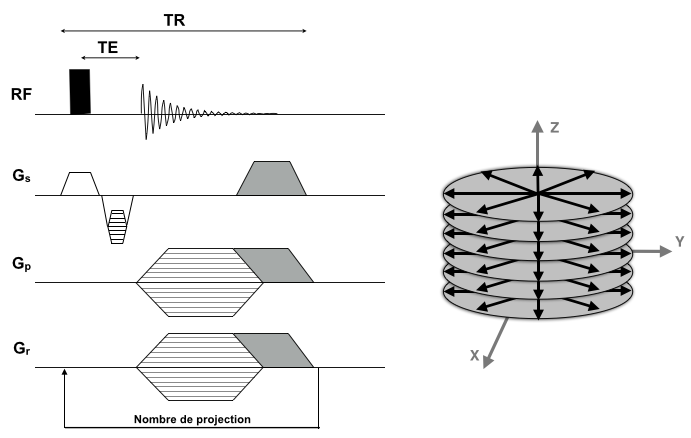
\includegraphics[scale=0.6]{./figure/chap2/KspaceStackOfUTE.png}
\caption[Chronogramme et trajectoire d'une séquence Stack-Of-Stars UTE.]{\label{fig:KspaceStackOfUTE} \textbf{Chronogramme et trajectoire d'une séquence Stack-Of-Stars UTE.} (a) Chronogramme d'une séquence radiale Stack-Of-Stars UTE. (b) Trajectoire d'une séquence Stack-Of-Stars UTE dans l'espace de Fourier. } 
\line(1,0){400} \\
\end{figure}

\subsection{Reconstruction}

\label{subsec:reconstruction}
Différentes approches sont utilisées pour la reconstruction des acquisitions radiales : la rétro-projection filtrée, le remaillage (gridding) ou la FFT non uniforme (nuFFT). Dans cette partie, c'est la reconstruction par remaillage qui sera détaillée puisque c'est cette dernière qui est la plus communément utilisée et qui a été appliquée pour ces travaux de thèse.

La méthode de reconstruction par remaillage a été introduite en imagerie médicale par O'Sullivan en 1985 \cite{o1985fast} et fut plus tard appliquée à la reconstruction d'images IRM recueillies avec des trajectoires d'acquisitions non-cartésiennes. Cette technique consiste à interpoler les points échantillonnés sur une grille rectilinéaire avant d'effectuer une reconstruction avec l'algorithme de FFT (figure \ref{fig:Gridding}).

\begin{figure}[h]
\centering
\line(1,0){400} \\
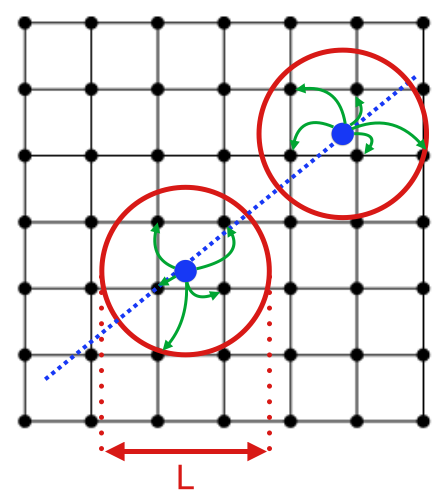
\includegraphics[scale=0.6]{./figure/chap2/Gridding.png}
\caption[Interprétation graphique de l'opération de remaillage.]{\label{fig:Gridding} \textbf{Interprétation graphique de l'opération de remaillage.} L'opération de remaillage consiste à déterminer quels points de la grille cartésienne (en noir) sont contenus autour d'un point échantillonné (en bleu) à une distance inférieure à $\frac{L}{2}$. La distance séparant chacun des points de la grille au point échantillonné est utilisée comme paramètre $d$ dans le kernel.} 
\line(1,0){400} \\
\end{figure}

Dans le cas de l'imagerie radiale, la densité de points variable dans l'espace de Fourier nécessite d'être compensée \textit{a priori} ou \textit{a posteriori} de l'interpolation. Généralement, la fonction de compensation en densité est utilisée comme un poids attribué à chaque point de l'espace de Fourier échantillonné. Pour disposer les points sur une grille cartésienne, le signal mesuré est convolué avec un kernel d'interpolation. La littérature a montré que l'utilisation d'un kernel Kaiser-Bessel est optimale pour l'opération d'interpolation des données pour les acquisitions radiales. Celui-ci permet d'optenir des images de bonne qualité avec une taille du kernel $L$ raisonnable et est défini par :
\begin{equation}
  K_{kb}(d) = \left\{
      \begin{aligned}
         \frac{1}{L}I_0(\beta \sqrt{1-(2d/L)^2}) \;\;\;\;\;\;  |d| \leq \frac{L}{2}\\
	     0 \;\;\;\;\;\; |d| \leq \frac{L}{2}
      \end{aligned}
    \right.
\end{equation}
où $L$ correspond à la taille du kernel, d à la distance séparant le point à remailler d'un point de grille, $\beta$ est un facteur de forme et $I_0$ correspond à la fonction de Bessel modifiée de première d'espèce d'ordre 0.
La taille du kernel $L$ impacte la qualité des images reconstruites; plus grande sera sa taille plus l'image sera de bonne qualité. Cependant cela influera fortement sur le temps de reconstruction pour un gain potentiellement faible en qualité. Une valeur de 2 à 4 est généralement utilisée car elle permet d'obtenir une image avec une bonne qualité tout en limitant le temps de reconstruction. Le facteur $\beta$ est sélectionné en accord avec l'équation décrite par Beatty et al. \cite{Beatty:2005fk}. La forme du kernel est représentée dans la figure \ref{fig:KaiserBessel}.
\begin{figure}[H]
\centering
\line(1,0){400} \\
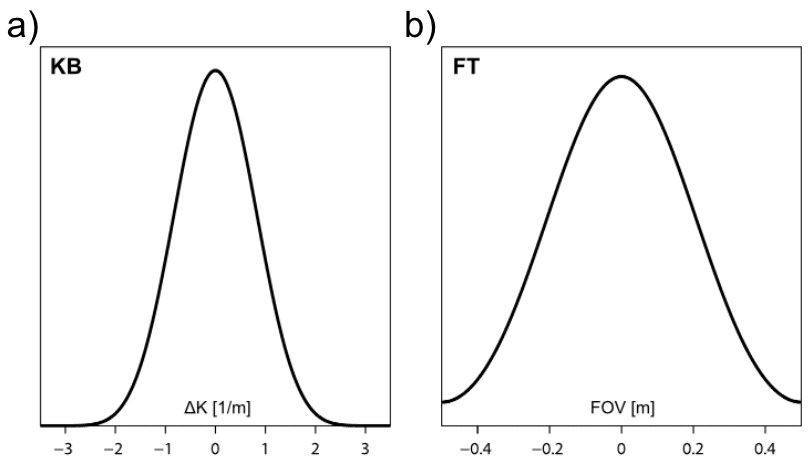
\includegraphics[scale=0.6]{./figure/chap2/KaiserBessel.png}
\caption[Représentation du filtre kernel Kaiser-Bessel.]{\label{fig:KaiserBessel} \textbf{Représentation du filtre kernel Kaiser-Bessel.} (a) Représentation dans le domaine de l'espace de Fourier du filtre kernel Kaiser-Bessel pour une valeur de $L = 6$ et $\beta = 13,8551$, où le champ de vue est normalisé à 1 m. (b) Représentation du kernel présenté en a) dans le domaine image par une transformée de Fourier .}
\line(1,0){400} \\
\end{figure}

Malheureusement la convolution avec un kernel d'une taille finie entraîne sur l'image obtenue après FFT des artefacts de modulation appelés effets roll-off (figure \ref{fig:deapod}). Cette modulation d'intensité de signal peut être compensée en divisant l'image par la transformée de Fourier du kernel qui est approximée par l'équation :
\begin{equation}
	FFT[K_{KB}](d) = \frac{\sin(\sqrt{(\pi L d)^2-\beta^2})}{\sqrt{(\pi L d)^2-\beta^2}}
\end{equation}
La convolution avec un kernel fini a aussi pour effet de créer des lobes secondaires qui sont repliés sur l'image.  Bien que l'amplitude initiale de ces lobes soit généralement faible avec un choix de kernel approprié, leurs intensités sont amplifiées par la correction de l'effet roll-off. Une solution simple à ce problème consiste à augmenter le champ de vue en effectuant le gridding sur une matrice plus grande, généralement d'un facteur 2. L'augmentation du champ de vue est ensuite corrigée en utilisant seulement les pixels centraux de l'image correspondant au champ de vue utilisé.

\begin{figure}[H]
\centering
\line(1,0){400} \\
\includegraphics[scale=0.6]{./figure/chap2/deapod.png}
\caption[ Correction de l'effet Roll-Off.]{\label{fig:deapod}\textbf{ Correction de l'effet Roll-Off.} Effet de la correction de l'effet Roll-Off sur un fantôme. La variation de signal entre le centre et les bords du fantôme est compensée par la division avec la transformée de Fourier du kernel utilisé pour le remaillage. Figure extraite d'une présentation de Otazo R. \cite{otazo:2014Reconstructi} .}
\line(1,0){400} \\
\end{figure}

La procédure de remaillage se compose donc des étapes suivantes :
\begin{enumerate}
\item Compensation en densité
\item Interpolation sur une grille par convolution avec un kernel
\item FFT
\item Correction de l'effet roll-off
\item Découpe de l'image
\end{enumerate}

\subsection{Avantages et désavantages de la trajectoire radiale}

La trajectoire radiale offre des propriétés uniques du fait de sa géométrie ou de l'ordonnancement de l'acquisition de l'espace de Fourier. Certaines de ces propriétés sont avantageuses par rapport à une acquisition cartésienne mais d'autres peuvent se transformer en inconvénients. Dans cette section, nous discuterons de ces propriétés en gardant en vue les applications possibles.
 
\subsubsection{Fonction d'étalement du point}

Pour comprendre les caractéristiques de n'importe quel système d'imagerie, il est souvent très intéressant d'étudier la fonction d'étalement du point (Point Spread Function : PSF). La PSF décrit la réponse du système à une impulsion (un dirac) et permet d'apprécier la façon dont un objet est imagé par celui-ci. En IRM, la PSF est fortement liée à la trajectoire utilisée dans l'espace de Fourier. En ignorant les phénomènes de relaxation pour plus de simplicité, la PSF d'une séquence IRM peut être obtenue en reconstruisant une image avec des données égales à 1 suivant la trajectoire radiale.

La figure \ref{fig:PSF} présente : a) les PSFs obtenues en fonction de $n_p$ le nombre de projections en imagerie UTE et b) les images correspondantes acquises sur un thorax de souris avec une résolution de base de $n = 128$ pixels. D'après l'équation \ref{eq:NyquistRad}, pour la résolution de 128 pixels, il est nécessaire pour une acquisition UTE de recueillir 402 projections. Dans ce cas, on observe un pic au centre de la PSF bien distinct qui est entouré par des oscillations circulaires mineures dont les amplitudes diminuent en s'écartant du centre. Ces oscillations sont dues à l'utilisation d'un espace de Fourier fini, et sont à l'origine d'un effet dit de troncature. Si l'on diminue le nombre de projections $n_p$ utilisé pour la reconstruction, par exemple à 134 projections, on peut voir qu'une démarcation apparaît dans la PSF à une certaine distance du centre de l'espace de Fourier (double flèches blanches). Cette distance définie ainsi la taille d'une région sans artefact \cite{Scheffler:1998fk} et en dehors de laquelle des artefacts de "streaking" apparaissent De plus, la largeur à mi-hauteur du pic central est plus large ce qui traduit une légère diminution de la résolution. Chaque "point" de l'objet étant convolué avec la PSF durant la reconstruction, le motif de "streaking" apparaît sur l'image reconstruite à une distance correspondant à la taille de cette région sans artefact dans la PSF. Lorsque l'on réduit le nombre de projections utilisé, le diamètre de cette région diminue et les artefacts sont plus prononcés. Cela est particulièrement visible sur la PSF et l'image reconstruite avec 40 projections.
En 3D, les artefacts de "streaking" sont plus diffus ce qui se traduit plutôt comme un bruit sur l'image et permet donc un sous-échantillonnage plus important de l'espace \cite{Gu:2005aa}.

\begin{figure}[h]
\centering
\line(1,0){400} \\
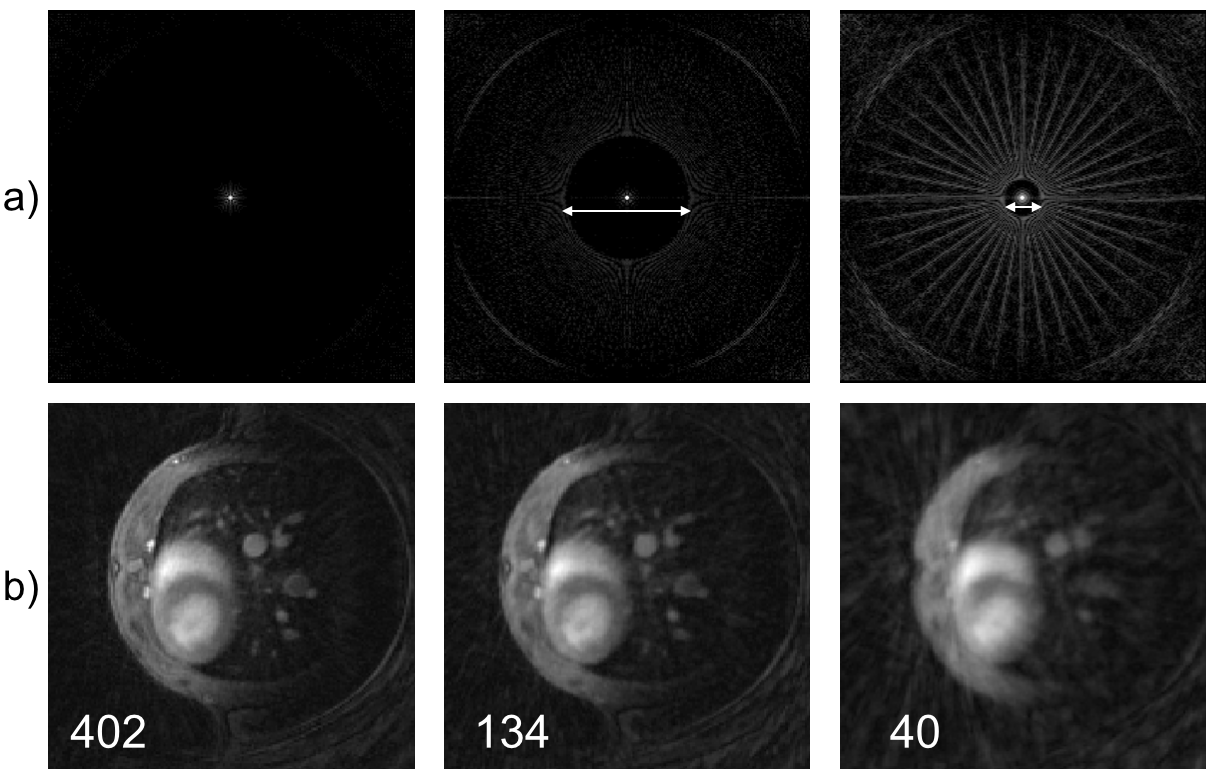
\includegraphics[scale=0.4]{./figure/chap2/PSF.png}
\caption[Effet du sous-échantillonnage sur la fonction d'étalement du point.]{\label{fig:PSF} \textbf{Effet du sous-échantillonnage sur la fonction d'étalement du point.} a) Représentation des PSFs dans le plan reconstruites à partir d'une trajectoire UTE 2D avec 402, 134 et 40 projections (résolution de base : 128 pixels) (b) Reconstruction des images correspondantes acquises sur un thorax de souris. Les flèches blanches montrent le diamètre correspondant au champ de vue sans artefacts.}
\line(1,0){400} \\
\end{figure}

Par rapport à une trajectoire cartésienne, le nombre de lignes de l'espace de Fourier à recueillir est supérieur pour respecter le critère de Nyquist, ce qui augmente \textit{a priori} le temps d'acquisition requis pour les séquences radiales. En pratique, il est néanmoins tout à fait possible de recueillir un nombre plus restreint de projections. Cela vient du fait que la région d'intérêt est souvent positionnée à l'intérieur de l'objet et donc que la présence d'artefacts de "streaking" aux bords de l'image peut ne pas gêner l'interprétation ou la quantification. Puisque la région centrale de la PSF est faiblement affectée par le nombre de projections utilisé, la trajectoire radiale offre une intéressante possibilité de sous-échantillonnage de l'espace de Fourier. Contrairement à l'acquisition cartésienne où une réduction du nombre de lignes recueillies aura pour conséquence une importante perte en résolution ou l'apparition d'artefacts de repliement rendant l'image inutilisable, avec une trajectoire radiale, la plupart des informations restent visibles malgré la nette présence d'artefact de "streaking".

\subsubsection{Distribution des points échantillonnés}

En imagerie radiale, puisque toutes les projections passent par le centre du plan de Fourier, le nombre de points échantillonnés est plus important pour les basses fréquences de l'espace de Fourier que pour les hautes fréquences. Cela est très différent des acquisitions cartésiennes où toutes les fréquences sont couvertes de la même façon. Bien que le fait d'avoir une distribution variable de points échantillonnés dans l'espace de Fourier implique quelques difficultés pour la reconstruction (voir section \ref{subsec:reconstruction}), cela peut néanmoins devenir avantageux pour la plupart des objets à imager. En effet, la plupart des images du monde réel sont caractérisées par une concentration en énergie près du centre de l'espace de Fourier, cela est aussi bien valable pour les images médicales de tomographie que pour les autres images naturelles \cite{srivastava2003advances}. C'est pourquoi il est intéressant de mesurer les basses fréquences plus "précisément" même au détriment du nombre de points échantillonnés dans les régions périphériques de l'espace de Fourier contenant moins d'informations. 

Des images avec une faible résolution peuvent être reconstruites à partir d'une partie des projections recueillies. Cela est possible car le nombre de points échantillonnés est suffisamment dense au centre de l'espace de Fourier pour satisfaire le critère de Nyquist et obtenir une image sans artefact comme expliqué dans la section précédente. De nombreuses applications peuvent alors être envisagées, par exemple en 2D, une série d'images résolues dans le temps peuvent être extraites d'un jeu de donnée complet pour identifier et corriger des artefacts de mouvement qui peuvent survenir durant l'acquisition.

Une caractéristique supplémentaire de la géométrie radiale est que chaque projection apporte autant d'information sur les basses et hautes fréquences, alors qu'avec une acquisition cartésienne, les informations de basses fréquences ne sont contenues que dans quelques lignes. Cela fait de l'imagerie radiale une option attractive quand une mise à jour continue de l'image est importante, par exemple en imagerie interventionnelle (\cite{Peters:2004aa} ou bien pour de la prise de contraste dynamique \cite{Prieto:2010oq}). Récemment, une méthode alternative nommée "Highly Constrained Backprojection" utilise ce rafraîchissement constant de l'image durant l'injection d'un agent de contraste. Cette méthode autorise des sous-échantillonnages très importants et assure une forte résolution temporelle tout en gardant une bonne résolution spatiale \cite{Wu:2011vn,Grist:2012fk}.

\subsubsection{Mouvements et flux}
\label{subsec:MouvEtFlux}
L'avantage le plus important d'une acquisition radiale réside dans sa faible sensibilité aux mouvements comparé aux séquences cartésiennes. Ceci s'explique principalement par deux raisons. La première est que cette sensibilité est une conséquence de la propriété de translation de la transformée de Fourier : un mouvement dans le domaine image se traduit par une modulation de la phase dans l'espace de Fourier. La forme de cette modulation dépend du type de mouvement et dans la littérature on distingue généralement des mouvements périodiques, pulsatiles ou ayant une vitesse constante \cite{Glover1991Phase-offset-mu}. Bien que ces mouvements soient différents, ils causent tous l'apparition du même type d'artefact qui sont des copies des parties mouvantes à d'autres positions dans l'image. Ces artefacts apparaissent exclusivement dans la direction d'encodage de phase ou de coupe et selon le type de mouvement peuvent créer une ou plusieurs copies qui peuvent gêner l'interprétation. 

\begin{figure}[h]
\centering
\line(1,0){400} \\
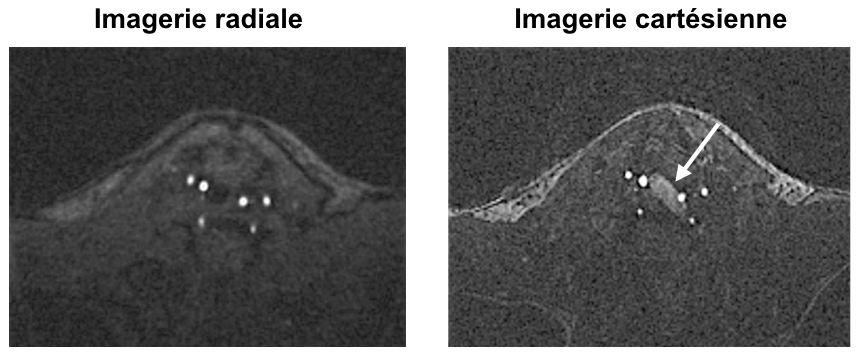
\includegraphics[scale=0.5]{./figure/chap2/Fig14.png}
\caption[Mouvements et imagerie radiale.]{\label{fig:MotionArt} \textbf{Mouvements et imagerie radiale.} Vues axiales des carotides d'une souris obtenues avec une séquence 3D cartésienne à droite et avec une séquence 3D PR à gauche. La flèche montre un artefact de flux sur l'image cartésienne qui correspond à une copie de la crosse aortique.}
\line(1,0){400} \\
\end{figure}

En imagerie radiale, les artefacts de mouvement se traduisent par du flou ou des artefacts de "streaking" qui se propagent perpendiculairement à la direction de lecture et qui sont éloignés de l'objet en mouvement d'une certaine distance, ce qui disperse l'erreur de manière plus ou moins homogène. Cette dispersion est encore plus efficace pour les séquences radiales 3D que 2D. Ces artefacts sont généralement moins dérangeants pour le diagnostic que les artefacts apparaissant en imagerie cartésienne (figure \ref{fig:MotionArt}).
Une deuxième raison expliquant la faible sensibilité aux mouvements pour l'imagerie radiale repose sur le sur-échantillonnage du centre de l'espace de Fourier grâce auquel un moyennage des projections contrebalance les erreurs enregistrées durant les phases de mouvement.
Ces deux propriétés réunies permettent d'expliquer le fort engouement des séquences 3D radiales pour l'imagerie d'organes en mouvement ou de patients peu coopératifs comme en pédiatrie \cite{block2014towards,Nayak:2014aa}.
Les séquences UTE bénéficient enfin d'un autre avantage car, après l'excitation, les spins sont déphasés puis rephasés par moins de gradient qu'avec des séquences cartésiennes. Cela permet de limiter les artefacts de déphasage de flux qui se traduisent par une absence de signal (figure \ref{fig:FluxArt}).

Pour toutes ces raisons, l'utilisation de séquences radiales est un choix intéressant en particulier pour des applications en angiographie et sur le petit animal. 
\begin{figure}[H]
\centering
\line(1,0){400} \\
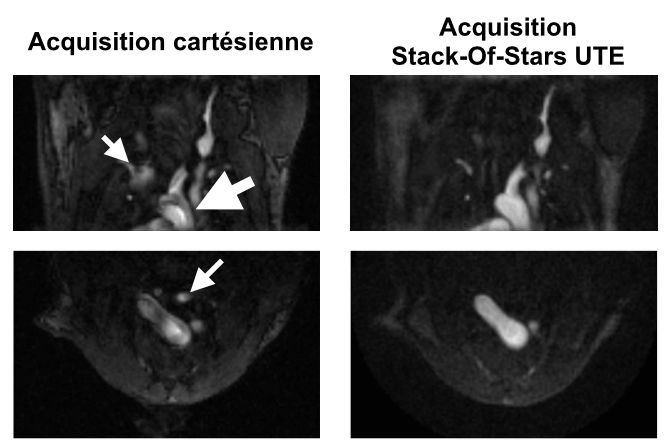
\includegraphics[scale=0.5]{./figure/chap2/Fig13.png}
\caption[Flux et imagerie radiale.]{\label{fig:FluxArt} \textbf{Flux et imagerie radiale.} Vue coronale (en haut) et axiale (en bas) de la crosse aortique d'une souris obtenues avec une séquence 3D cartésienne à gauche et avec une séquence 3D Stack-Of-Stars UTE à droite. Les deux acquisitions ont été effectuée sans synchronisation cardiaque ou respiratoire. La flèche épaisse montre une inhomogénéité du signal dans la crosse aortique qui sont des artefacts de déphasage du flux et les autres flèches  des artefacts de mouvement.}
\line(1,0){400} \\
\end{figure}

\subsubsection{Sur-échantillonnage en lecture}

Puisque l'espace de Fourier est échantillonné de manière discrète en IRM, la reconstruction de l'objet est périodique. C'est pour cela que l'on observe des effets de repliements de l'image si les points échantillonnés sont trop distants dans l'espace de Fourier et que les copies voisines se chevauchent dans le domaine image. Pour une résolution spatiale fixée, ce problème peut être éliminé en suréchantillonant la lecture, c'est-à-dire en utilisant une bande passante de réception plus grande. Cela permet donc d'augmenter le champ de vue mais aussi de compenser la diminution du rapport signal-sur-bruit induite par l'augmentation de la bande passante.

Pour l'imagerie cartésienne, cette possibilité de sur-échantillonnage est limitée à la direction de lecture car une augmentation du nombre de points dans les autres directions nécessitera l'acquisition de lignes supplémentaires. Pour l'imagerie radiale, cette limitation n'existe pas et le sur-échantillonnage peut être employé dans toutes les directions. C'est une particularité particulièrement  intéressante pour l'imagerie abdominale ou cardiaque \cite{block2014towards,Johnson:2012uq} où les régions d'intérêts sont localisées au centre. Cela permet de réduire le champ de vue nécessaire et donc de réduire le temps d'acquisition.

\begin{figure}[H]
\centering
\line(1,0){400} \\
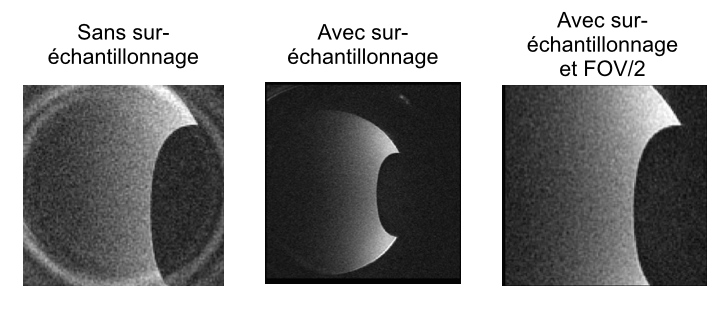
\includegraphics[scale=0.7]{./figure/chap2/Oversampling.png}
\caption[Effet du suréchantillonnage en lecture.]{\label{fig:Oversampling} \textbf{Effet du suréchantillonnage en lecture.} Vue axiale d'un fantôme. A gauche : Image acquise avec une séquence UTE sans sur-échantillonnage en lecture (Nombre de points recueillis = 70 et bande passante de réception = 100 kHz). Au centre : Image acquise avec une séquence UTE avec sur-échantillonnage en lecture (Nombre de points receuillis = 140 et bande passante de réception = 200 kHz). A droite : Seul la partie de centrale de l'image du centre est conservée pour correspondre au champ de vue désirée. On observe que l'artefact en cercle n'est plus présent sur l'image avec sur-échantillonnage ainsi qu'une amélioration du rapport signal-sur-bruit grâce à l'absence de repliement avec un champ de vue deux fois plus grand.}
\line(1,0){400} \\
\end{figure}

\subsubsection{Déviations des gradients}

Au cours des acquisitions IRM, les gradients de champ magnétique doivent rapidement monter puis descendre en intensité à de multiples reprises ce qui implique la création de courants de Foucault dans les bobines. Cela va modifier la trajectoire d'échantillonnage des points dans l'espace de Fourier.
Pour les séquences cartésiennes, cela ne pose pas de problème majeur car des formes de gradients identiques sont générées dans la direction de lecture pour toutes les répétitions. Cela résultera durant la reconstruction à une translation de la position des points échantillonnés selon la direction de lecture et donc à une modulation de phase dans le domaine image qui disparaîtra lorsque l'image en magnitude sera calculée.

Cela est différent pour l'imagerie radiale car la direction de lecture varie pour chaque répétition. Dans cette situation, un simple délai de réponse des gradients cause une erreur non-uniforme de positionnement des points. Cela se traduit par des pertes de signal et du flou dans les images. C'est pour cela qu'il est nécessaire d'utiliser des méthodes de correction. Différentes techniques ont été proposées \cite{Alley:1998vn,Addy:2012kx} mais la méthode utilisée durant ces travaux de thèse est celle originellement décrite par Zhang et al \cite{Zhang:1998uq}. Elle a l'avantage d'être simple à mettre en oeuvre.
Celle-ci consiste à mesurer le signal dans deux coupes positionnées symétriquement par rapport à l'isocentre, perpendiculairement à la direction du gradient. La phase du signal est extraite du signal puis déroulée pour éviter les repliements. La trajectoire dans l'espace selon cette axe est alors calculée en utilisant la phase des deux coupes. Cette méthode est reproduite sur chaque axe pour obtenir les trajectoires dans la $2^\text{ème}$ ou $3^\text{ème}$ dimension selon la séquence. Le chronogramme, la position des coupes et l'algorithme sont présentés dans la figure \ref{fig:SeqTraj}.

\begin{figure}[H]
\centering
\line(1,0){400} \\
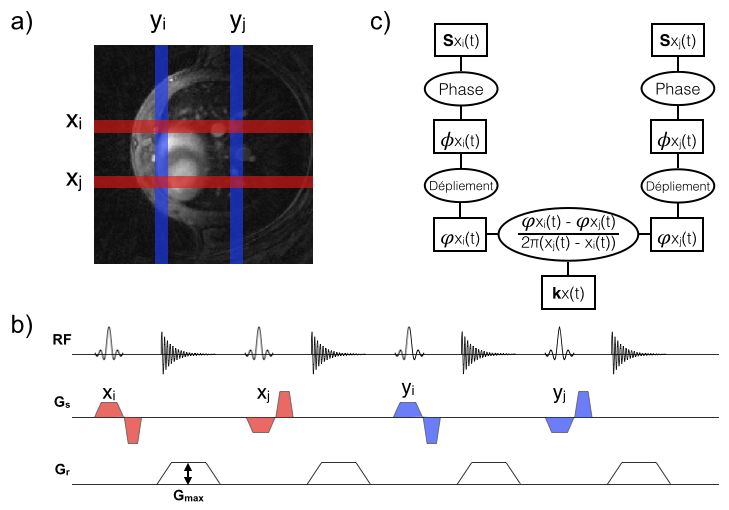
\includegraphics[scale=0.6]{./figure/chap2/SeqTraj.png}
\caption[Méthode de mesure des trajectoires 2D.]{\label{fig:SeqTraj}  
\textbf{Méthode de mesure de trajectoire 2D UTE} : (a) Positionnement des coupes de mesure symétriques par rapport à l'isocentre. (b) Chronogramme de la séquence utilisée. (c) Diagramme décrivant l'algorithme utilisé pour obtenir la trajectoire de l'axe vertical dans l'espace de Fourier à partir du signal dans les coupes $x_i$ et $x_j$.}
\line(1,0){400} \\
\end{figure}

\subsubsection{Sensibilité aux effets d'Off-Résonance}

En imagerie radiale les artefacts d'off-résonance sont différents de ceux en imagerie cartésienne. La variation d'évolution de la phase cause un déplacement des informations spatiales selon chaque orientation des projections qui crée donc un flou dans l'image (figure \ref{fig:OffRes}).
On peut distinguer plusieurs sources d'artefacts (la graisse, les effets de susceptibilité, l'inhomogénéité du champ statique, etc). La correction de ces artefacts \textit{a posteriori} n'est pas triviale et une stratégie plus rationnelle consiste à les réduire en modifiant la méthode d'acquisition avec :
\begin{enumerate}
\item une augmentation de la bande passante de réception
\item l'utilisation de séquence à temps d'écho court
\item l'utilisation de séquence de type Echo de Spin
\end{enumerate}

Généralement, la principale source d'artefact d'off-résonance est la présence de graisse. En imagerie cardiovasculaire sur petit animal, la graisse est peu présente autour des zones d'intérêt comme le cœur, la crosse aortique ou les carotides ce qui limite les artefacts. Cependant pour des méthodes nécessitant de longs temps d'écho, par exemple, pour obtenir un contrast $T_2^*$, l'imagerie radiale n'est pas conseillée et il est alors préférable d'utiliser une approche cartésienne ou bien une méthode de suppression de graisse (saturation, excitation sélective etc).
\begin{figure}[H]
\centering
\line(1,0){400} \\
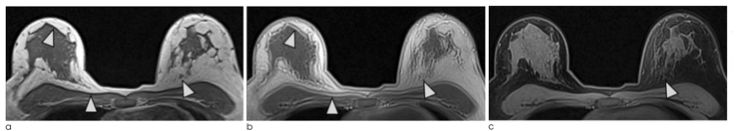
\includegraphics[scale=0.7]{./figure/chap2/OffRes.png}
\caption[Illustration des artefacts de déplacement chimique en imagerie radiale.]{\label{fig:OffRes}  \textbf{Illustration des artefacts de déplacement chimique en imagerie radiale.}
(a) En imagerie cartésienne, la présence de graisse crée un artefact de déplacement chimique dans la direction de lecture. (b) A cause de la modification de l'orientation de la direction de lecture en imagerie radiale, les artefacts apparaissent comme un flou entourant les zones graisseuses. (c) Ces artefacts peuvent être éliminés en utilisant une méthode de suppression de graisse. Figure extraite d'un article de Block et Al. \cite{block2014towards}}.
\line(1,0){400} \\
\end{figure}

\section{Résumé}

Avec un schéma d'acquisition radiale, les données de l'espace de Fourier sont recueillies selon des projections plutôt que des lignes parallèles. La modification d'une séquence cartésienne existante en une séquence radiale peut généralement être facilement effectuée que ce soit en 2D ou en 3D. Cependant, à cause de la position non équidistante des points, une méthode de reconstruction spéciale doit être utilisée comme le remaillage des données.

L'imagerie radiale dispose de plusieurs avantages par rapport à une acquisition cartésienne comme une faible sensibilité aux artefacts de flux et de mouvement, la possibilité de sur-échantillonner l'acquisition dans toutes les directions sans augmenter le temps d'acquisition requis ce qui élimine les artefacts de repliement. De plus, le centre de l'espace de Fourier est sur-échantillonné en termes de nombre de projections, ce qui autorise alors un sous-échantillonnage de l'acquisition. Bien que l'acquisition d'un nombre réduit de projections puissent créer des artefacts de "streaking", une grande partie des informations de l'objet reste visible même avec un fort facteur d'accélération, ce qui n'est pas le cas avec une trajectoire cartésienne. De plus, chaque projection acquiert un niveau équivalent d'information de hautes et de basses fréquences, ce qui offre une mise à jour des informations plus homogène pour des applications en temps réel ou dynamique en IRM.

D'un autre côté, le nombre de projections à recueillir pour obtenir un espace de Fourier complet est plus important qu'en imagerie cartésienne ce qui peut prolonger le temps d'acquisition. L'imagerie radiale est aussi plus sensible aux déviations des valeurs des gradients, bien qu'aujourd'hui cela soit un problème moins important avec les systèmes récents d'IRM. Le principal problème de cette méthode est sa sensibilité aux artefacts de déphasage et en particulier de déplacement chimique. C'est pourquoi l'utilisation de séquence radiale n'est pas recommandée pour obtenir un contraste $T_2^*$.

